% Arquitectura en TikZ, fuente vectorial de la figura 5.1.
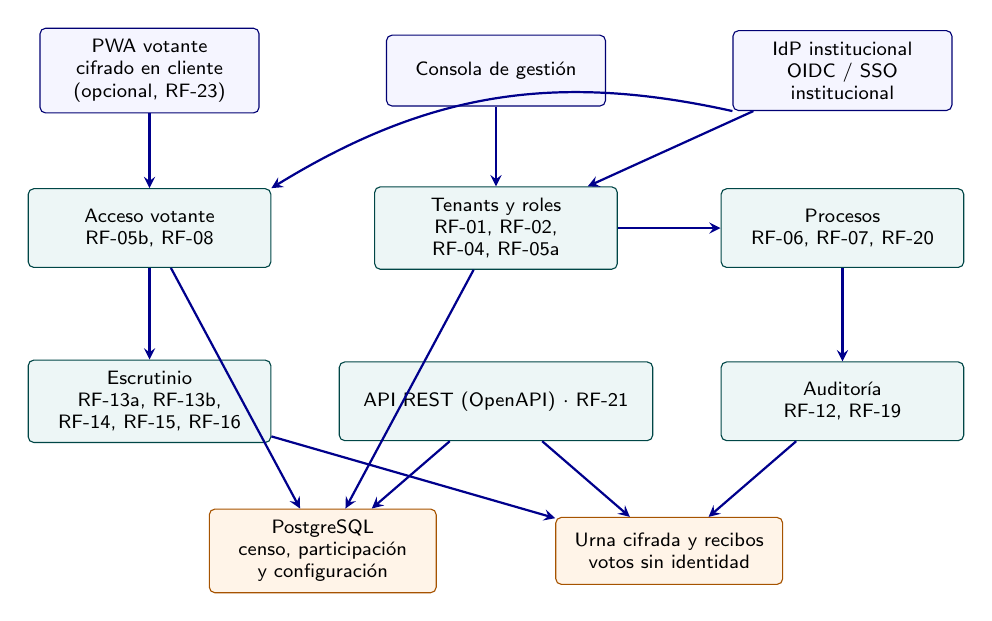
\begin{tikzpicture}[
  font=\sffamily\scriptsize,
  box/.style={draw=blue!45!black, rounded corners=2pt, fill=blue!4,
    align=center, minimum height=0.9cm, text width=2.5cm, inner sep=4pt},
  mod/.style={draw=teal!55!black, rounded corners=2pt, fill=teal!7,
    align=center, minimum height=1cm, text width=2.8cm, inner sep=4pt},
  store/.style={draw=orange!65!black, rounded corners=2pt, fill=orange!9,
    align=center, minimum height=0.85cm, text width=2.6cm, inner sep=4pt},
  link/.style={->,>=stealth, thick, draw=blue!55!black},
  optional/.style={->,>=stealth, dashed, thick, draw=gray!75}
]
\node[box] (pwa) at (0,0) {PWA votante\\cifrado en cliente (opcional, RF-23)};
\node[box] (gest) at (4.4,0) {Consola de gestión};
\node[box] (idp) at (8.8,0) {IdP institucional\\OIDC / SSO institucional};

\node[mod] (access) at (0,-2.0) {Acceso votante\\RF-05b, RF-08};
\node[mod] (tenant) at (4.4,-2.0) {Tenants y roles\\RF-01, RF-02, RF-04, RF-05a};
\node[mod] (election) at (8.8,-2.0) {Procesos\\RF-06, RF-07, RF-20};

\node[mod] (ballot) at (0,-4.2) {Escrutinio\\RF-13a, RF-13b, RF-14, RF-15, RF-16};
\node[mod,text width=3.7cm] (api) at (4.4,-4.2) {API REST (OpenAPI) $\cdot$ RF-21};
\node[mod] (audit) at (8.8,-4.2) {Auditoría\\RF-12, RF-19};

\node[store] (db) at (2.2,-6.1) {PostgreSQL\\censo, participación y configuración};
\node[store] (urn) at (6.6,-6.1) {Urna cifrada y recibos\\votos sin identidad};

\draw[link] (pwa) -- (access);
\draw[link] (gest) -- (tenant);
\draw[link] (idp) -- (tenant);
\draw[link] (idp.south west) to[bend right=22] (access.north east);
\draw[link] (access) -- (ballot);
\draw[link] (tenant) -- (election);
\draw[link] (election) -- (audit);
\draw[link] (ballot) -- (urn);
\draw[link] (access) -- (db);
\draw[link] (tenant) -- (db);
\draw[link] (api) -- (db);
\draw[link] (api) -- (urn);
\draw[link] (audit) -- (urn);
\end{tikzpicture}
